% \captionsetup{
%    tablename=TABELA,
%    listformat=empty,
%    justification=centering,
%    %labelsep=newline,
%    position=above,
%    skip=0.2\baselineskip,
%    width=\linewidth,
%    labelfont={small},
%    font={small} 
% }

\newcommand{\legenda}[1]{\caption{#1}}

\pagenumbering{arabic}

\def\BibTeX{{\rm B\kern-.05em{\sc i\kern-.025em b}\kern-.08em
    T\kern-.1667em\lower.7ex\hbox{E}\kern-.125emX}}

\newcommand{\tabelaname}{TABELA}
\newcommand{\figuraname}{FIGURA}
\newcommand{\quadroname}{QUADRO}
\newcounter{quadrocounter}
\setcounter{quadrocounter}{0}
% posicao, legenda, fonte
\newenvironment{quadro}[4][!t]
{
  \refstepcounter{quadrocounter}
  \label{#4}
  \def\fonteval{#3}
  \begin{table}[#1]
    \begin{center}
      % legenda
      \par\medskip\noindent
      QUADRO~\thequadrocounter~-~#2
      \par\medskip\noindent
}
{
      \par\noindent
      \fonte{\fonteval}
    \end{center}
  \end{table}
}
\newenvironment{quadro*}[4][!t]
{
  \refstepcounter{quadrocounter}
  \label{#4}
  \def\fonteval{#3}
  \begin{table*}[#1]
    \begin{center}
      % legenda
      \par\medskip\noindent
      QUADRO~\thequadrocounter~-~#2
      \par\medskip\noindent
}
{
      \par\noindent
      \fonte{\fonteval}
    \end{center}
  \end{table*}
}

\newcounter{tabelacounter}
\setcounter{tabelacounter}{0}
\newenvironment{tabela}[4][!t]
{
  \refstepcounter{tabelacounter}
  \label{#4}
  \def\fonteval{#3}
  \begin{table}[#1]
    \begin{center}
      % legenda
      \par\medskip\noindent
      TABELA~\thetabelacounter~-~#2
      \par\medskip\noindent
}
{
      \par\noindent
      \fonte{\fonteval}
    \end{center}
  \end{table}
}
\newenvironment{tabela*}[3][!t]
{
  \refstepcounter{tabelacounter}
  \def\fonteval{#3}
  \begin{table*}[#1]
    \begin{center}
      % legenda
      \par\medskip\noindent
      TABELA~\thetabelacounter~-~#2
      \par\medskip\noindent
}
{
      \par\noindent
      \fonte{\fonteval}
    \end{center}
  \end{table*}
}
\newcounter{figuracounter}
\setcounter{figuracounter}{0}
\newenvironment{figura}[4][!t]
{
  \def\fonteval{#3}
  \refstepcounter{figuracounter}
  \label{#4}
  \begin{figure}[#1]
    \begin{center}
      % legenda
      \par\medskip\noindent
      FIGURA~\thefiguracounter~-~#2
      \par\medskip\noindent
}
{
    \par\noindent
    \fonte{\fonteval}
    \end{center}
  \end{figure}
}
\newenvironment{figura*}[4][!t]
{
  \refstepcounter{figuracounter}
  \label{#4}
  \def\fonteval{#3}
  \begin{figure}[#1]
    \begin{center}
    % legenda
    \par\medskip\noindent
    FIGURA~\thefiguracounter~-~#2
    \par\medskip\noindent
}
{
    \par\noindent
    \fonte{\fonteval}
  \end{center}
  \end{figure}
}

\newcommand*{\captionsource}[2]{%
  \caption[{#1}]{%
  \centering
    #1%
    \hspace{\linewidth}%
    FONTE: #2%
  }%
}

\newcommand*{\fonte}[1]{%
  \centering
  \small
  \vspace{1em}
  \hspace{\linewidth}%
  FONTE: #1%
}

\def\abstractname{Abstract: }


%%%%%%%%%%%% CONFIGURAÇÃO DA CAPA E FOLHA DE ROSTO %%%%%%%%%%%%%%

\def\descr{Trabalho de conclusão de curso apresentado ao
curso de graduação em Análise e
Desenvolvimento de Sistemas, Setor de Educação
Profissional e Tecnológica, Universidade Federal
do Paraná, como requisito parcial à obtenção do
título de tecnólogo}



%%%% fundo na capa

\backgroundsetup{
scale=1,
color=black,
opacity=0.4,
angle=0,
contents={%
  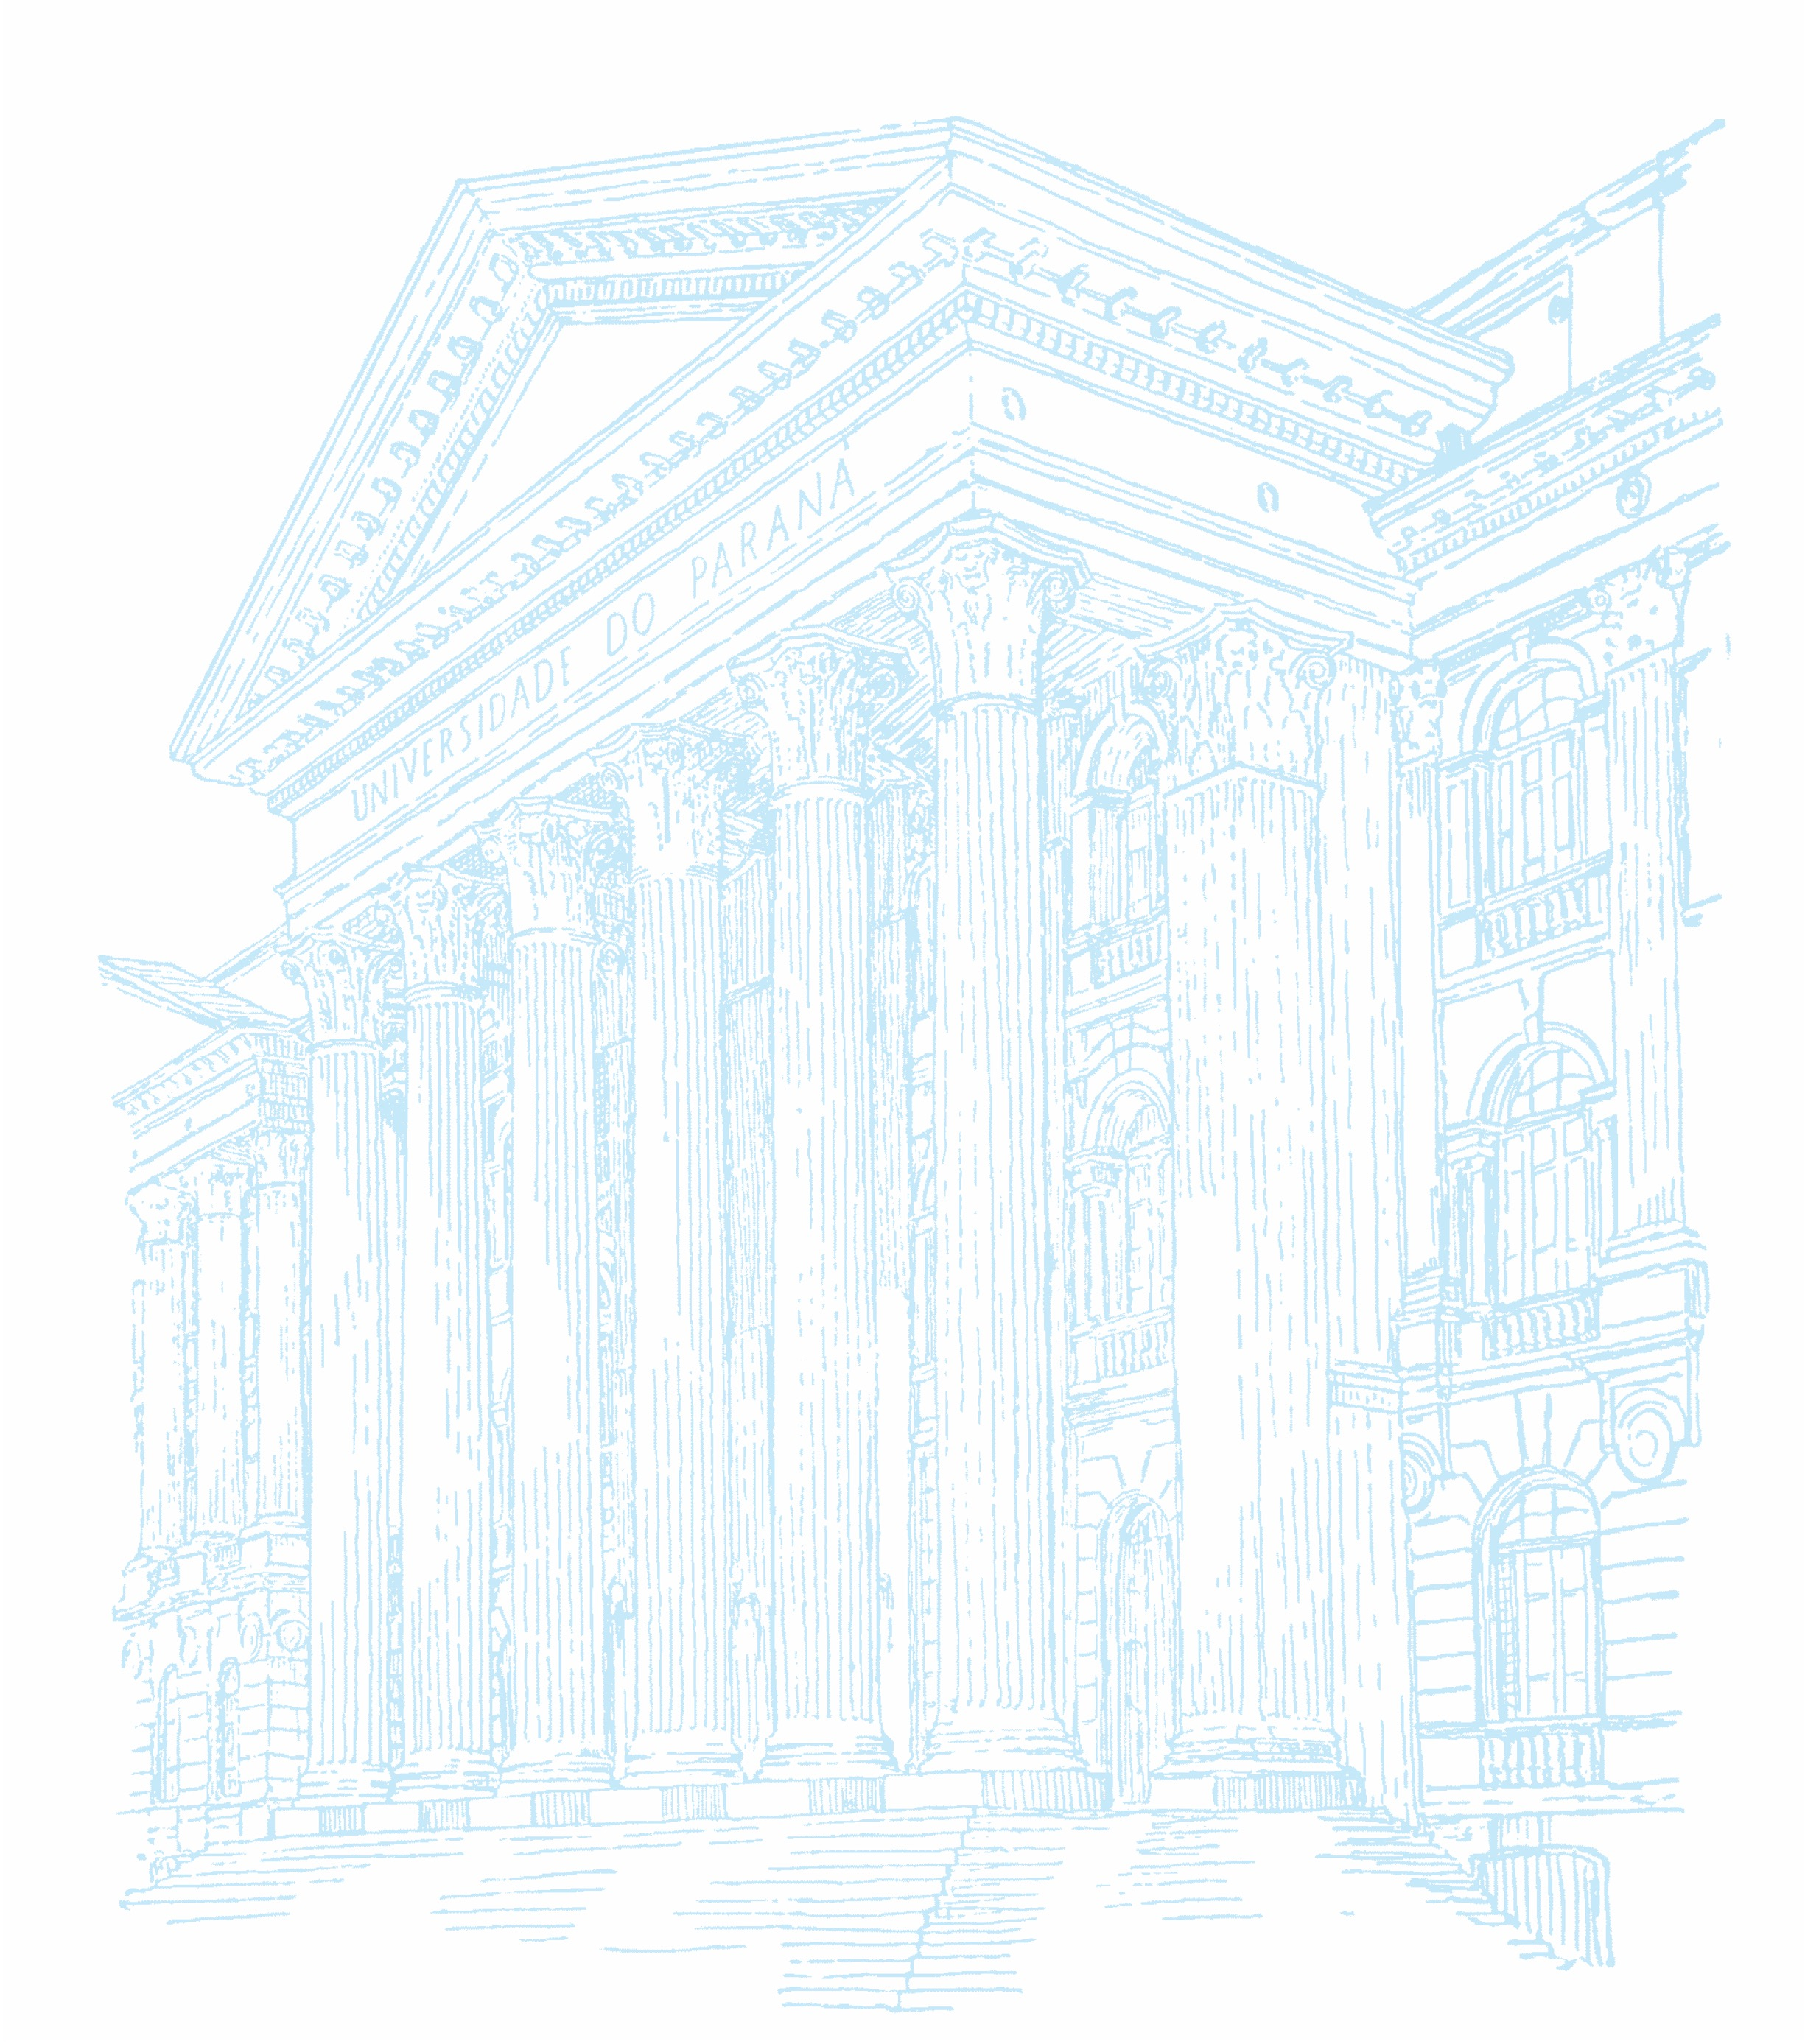
\includegraphics[width=\paperwidth,height=\paperheight]{bg_capa.jpg}
  }%
}
%%%%


%%%%%%% Definição da capa e folha de rosto


%\fancypagestyle{frontmatter}{
%  \fancyhf{}
%}

%\fancypagestyle{plain}{
%  \fancyhf{}
%  \if@mainmatter
%    \if@twoside
%      \fancyhead[LE,RO]{\thepage}
%    \else
%      \fancyhead[R]{\thepage}
%    \fi
%  \fi
%}



\hypersetup{
  % pdftitle, author, etc definidos mais abaixo
%  bookmarks   = true,
%  pageanchor  = false,
  hypertexnames = false,
%  bookmarkstype = page,
  pdfview     = Fit,
  pdfborder   = {0 0 0},
  colorlinks  = false,
  linkcolor   = blue,
  anchorcolor = blue,
  citecolor   = blue,
  filecolor   = blue,
%  pagecolor   = blue,
  urlcolor    = blue
}




%\def\@advisor{}			% orientador
%\def\@coadvisor{}		% co-orientador
%\def\@local{}			% local
%\def\@descr{}			% descrição do documento
%\def\@pcs{}			% palavras-chave
%\def\@kws{}			% keywords


%\newcommand{\autorcapa}[1]{\def\@author{#1}}
%\renewcommand{\title}[1]{\def\@title{#1}}

% descrição do documento na folha de rosto
%\newcommand{\descr}[1]{\def\@descr{#1}}

% orientadores
%\newcommand{\advisor}[1]{\def\@advisor{#1}}
%\newcommand{\coadvisor}[1]{\def\@coadvisor{#1}}


% local (cidade)
%\newcommand{\local}[1]{\def\@local{#1}}

\newcommand{\capa}[1]
{
  % páginas iniciais não são numeradas
  %\pagestyle{empty}
  %\thispagestyle{empty}

  % ajustar tags do PDF final
  \hypersetup{
    pdftitle    = {\titulo},
    pdfproducer = {UFPR - Universidade Federal do Paraná}
  }

  % primeira capa (só na versão aprovada)
  %\iffinalmode
%    \phantomsection
%    \thispagestyle{empty}

    \BgThispage
    
    \begin{center}
      \begin{doublespace}
        \textsc{\Large{UNIVERSIDADE FEDERAL DO PARANÁ}}
        \par
        \vspace{2cm}
        #1
        \vfill
        \DeclareRobustCommand\\{\linebreak}
        \textsc{\Large\titulo}
        \vfill
        \textsc{\Large\local\\\ano}
      \end{doublespace}
    \end{center}
    \cleardoublepage
    
    
  %\fi

  % folha de rosto
  \clearpage
%  \phantomsection
%  \addcontentsline{toc}{chapter}{Rosto}
%  \thispagestyle{empty}

  % autor
  \begin{center}
      \begin{doublespace}
        #1
      \end{doublespace}
  \end{center}

  \vfill\vfill

  % título
  \begin{doublespace}
    \begin{center}
      \DeclareRobustCommand\\{\linebreak }
      \textsc{\Large\titulo}
    \end{center}
  \end{doublespace}

  \vspace{1cm}

  % selo descritivo
  \hfill
  \begin{minipage}{9cm}

    % descrição
    \ifx\descr\@empty
    \else
      \descr.
    \fi

    % orientador
    \ifx\orientador\@empty
    \else
      \vspace{1em}
      Orientador: \orientadornome.
    \fi

    % coorientador
    \ifx\coorientador\undefined
    \else
      \vspace{1em}
      Co-orientador: \coorientador.
    \fi

  \end{minipage}

  \vfill

  % local e data
  \begin{center}
    \begin{doublespace}
      \textsc{\Large\local\\\ano}
    \end{doublespace}
  \end{center}

  % that's all, folks!
  \cleardoublepage
}


\newcommand{\termoaprovacao}
{
    \begin{center}
      \begin{doublespace}
        \vfill
        \Large{Substituir esta página pelo Termo de Aprovação que será fornecido após a defesa.}
        \vfill
      \end{doublespace}
    \end{center}
    \cleardoublepage
    
}

% \newcommand{\linebreakand}{%
%   \end{@IEEEauthorhalign}
%   \hfill\mbox{}\par
%   \mbox{}\hfill\begin{@IEEEauthorhalign}
% }

\newcommand*{\refmark}[1]{\raisebox{0pt}[0pt][0pt]{\textsuperscript{\footnotesize #1}}}
\newcommand{\autores}[1]{
  \author{
      \IEEEauthorblockN{
        #1
      }
      %\IEEEauthorblockN{#1\refmark{1}, #2\refmark{1}, #3\refmark{1}, #4\refmark{1}, #5\refmark{1}}
      \IEEEauthorblockA{\refmark{1}\textit{\setor} \\ \textit{\ufpr} }
  }
}

%%%%%%%
